
%!TEX encoding = UTF-8 Unicode
%!TEX root = ../exercises.tex

\ifPreSolution



\Exercise{\ExeWeekEIGHT}\label{exe:W08}

\begin{Goals}
\item Kunna skapa och använda matriser med nästlade strukturer av \code{Vector}.
\item Kunna iterera över elementen i en matris med nästlade \code{for}-satser och \code{for}-\code{yield}-uttryck, samt nästlad applicering av \code{map} respektive \code{foreach}.
\item Kunna skapa och använda funktioner som tar matriser som parametrar.
\item Känna till generiska funktioner.
\item Känna till generiska klasser.
\item Kunna skapa och använda matriser med hjälp inbyggda arrayer i Java.
\item Kunna använda nästlade \code{for}-satser i Java för att iterera över elementen i en matris.
\end{Goals}

\begin{Preparations}
\item \StudyTheory{08}
\end{Preparations}

\BasicTasks %%%%%%%%%%%%%%%%

\else



\ExerciseSolution{\ExeWeekEIGHT}

\BasicTasks %%%%%%%%%%%

%Uppgift 1

\fi





\WHAT{Skapa matriser med hjälp av nästlade samlingar.}

\QUESTBEGIN

\Task  \what~  Man kan i ett datorprogram, med hjälp av samlingar som innehåller samlingar, skapa nästlade strukturer som kan indexeras i två dimensioner och på så sätt representera en matematisk \textbf{matris}.\footnote{\href{https://sv.wikipedia.org/wiki/Matris}{sv.wikipedia.org/wiki/Matris}}
\begin{Background}
En \textbf{matris} inom matematiken innehåller ett antal rader och kolumner (även kallade kolonner). I en matematisk matris har alla rader lika många element och även alla kolumner har lika många element. En matris av dimension $m\times{}n$ har $m \cdot n$ stycken element, där $m$ är antalet rader och $n$ är antalet kolumner. En matris $A_{m,n}$ av dimension $m\times{}n$ ritas ofta så här:

\[
A_{m,n} =
 \begin{pmatrix}
  a_{1,1} & a_{1,2} & \cdots & a_{1,n} \\
  a_{2,1} & a_{2,2} & \cdots & a_{2,n} \\
  \vdots  & \vdots  & \ddots & \vdots  \\
  a_{m,1} & a_{m,2} & \cdots & a_{m,n}
 \end{pmatrix}
\]

\noindent Exempel: En heltalsmatris $M_{2,5}$ av dimension $2\times{}5$ där element $m_{2,5}=7$:

\[
M=
  \begin{pmatrix}
    5 & 2 & 42 & 4 & 5 \\
    3 & 4 & 18 & 6 & 7
  \end{pmatrix}
\]
\end{Background}

\Subtask\Pen Rita minnessituationen efter tilldelningen på rad 1 nedan. Vad har \code{m} för typ och värde? Vad har \code{m} för dimensioner? Hur sker indexeringen i ett datorprogram jämfört med i matematiken?

\begin{REPL}
scala> val m = Vector((1 to 5).toVector, (3 to 7).toVector)
scala> m.apply(0).apply(1)
scala> m(1)
scala> m(1)(4)
\end{REPL}

\Subtask Vad ger uttrycken på raderna 2, 3 och 4 ovan för värden och typ?

\Subtask Man kan i ett datorprogram mycket väl skapa tvådimensionella, nästlade strukturer där raderna \emph{inte} innehåller samma antal element. Det blir då ingen äkta matris i strikt matematisk mening, men man kallar ofta ändå en sådan struktur för en ''matris''. Vilken typ har variablerna \code{m2}, \code{m3}, \code{m4} och \code{m5} nedan?

\begin{REPL}
scala> val m2 = Vector(Vector(1,2,3),Vector(4,5),Vector(42))
scala> val m3 = Vector(Vector(1,2), Vector(1.0, 2.0, 3.0))
scala> m3(1)
scala> val m4 = m3(1) +: Vector("a") +: m3
scala> val m5 = Vector.fill(42){ m2(1).map(e => (e * math.random).toInt) }
\end{REPL}

\Subtask\Pen Rita minnessituationen efter tilldelingen av \code{m2} på rad 1 ovan.

\Subtask\Pen Vilken av variablerna \code{m2}, \code{m3}, \code{m4} och \code{m5} ovan representerar en äkta matris i matematisk mening? Vilken är dess dimensioner?



\SOLUTION


\TaskSolved \what


%1.a)
\SubtaskSolved   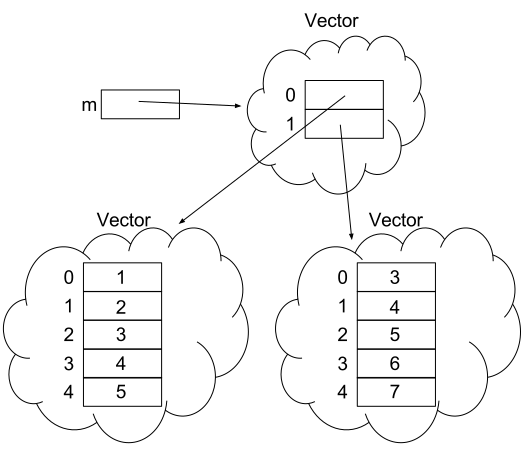
\includegraphics{../img/w09-solutions/1a} \\
Typ: \code{Vector[Vector[Int]]}\\
Värde: \code{Vector(Vector(1, 2, 3, 4, 5), Vector(3, 4, 5, 6, 7))} \\
Dimensioner: $2 \times 5$\\
Inom matematiken sker indexering enligt konvention med 1 som lägsta index. I scala är lägsta index 0, man använder s.k. 0-indexering. \footnote{Detta är inte fallet i alla programmeringsspråk, vilket du kan läsa mer om på \url{https://en.wikipedia.org/wiki/Array\_data\_type\#Index\_origin}}

%1. b)
\SubtaskSolved  \\
2: \code{Int}\\
3: \code{Vector[Int]}\\
4: \code{Int}

%1.c)
\SubtaskSolved  \\
m2: \code{Vector[Vector[Int]]}\\
m3: \code{Vector[Vector[AnyVal]]}\\
m4: \code{Vector[Vector[Any]]}\\
m5: \code{Vector[Vector[Int]]}

%1.d)
\SubtaskSolved  TODO

%1.e)
\SubtaskSolved  m5, $42 \times 2$



\QUESTEND




%%<AUTOEXTRACTED by mergesolu>%%      %Uppgift 2




\WHAT{Skapa och iterera över matriser.}

\QUESTBEGIN

\Task  \what~  Vi ska skapa matriser där varje rad representerar 5 kast med en tärning i spelet Yatzy.\footnote{\href{https://sv.wikipedia.org/wiki/Yatzy}{sv.wikipedia.org/wiki/Yatzy}}


\Subtask Definiera i REPL en funktion \code{def throwDie: Int = ???} som returnerar ett slumptal mellan 1 och 6.


\Subtask Skapa nedan heltalsmatris i REPL. Vilken dimension får matrisen?
\begin{REPL}
val ds1 = for (i <- 1 to 1000) yield {
            for (j <- 1 to 5) yield throwDie
          }
\end{REPL}

\Subtask\Pen Man kan också använda nedan varianter för att skapa en heltalsmatris. Vilken av varianterna \code{ds1} ... \code{ds5} tycker du är lättast att läsa och förstå? Prova respektive variant i REPL och ange vilken typ på \code{ds1} ... \code{ds5} som härleds av kompilatorn.
\begin{REPL}
val ds2 = (1 to 1000).map(i => (1 to 5).map(j => throwDie))
val ds3 = (1 to 1000).map(i => Vector.fill(5)(throwDie))
val ds4 = for (i <- 1 to 1000) yield Vector.fill(5)(throwDie)
val ds5 = Vector.fill(1000)(Vector.fill(5)(throwDie))
\end{REPL}


\Subtask Definiera en funktion \\ \code{def roll(n: Int): Vector[Int] = ???}\\ som ger en heltalsvektor med $n$ stycken slumpvisa tärningskast. Kasten ska vara sorterade i växande ordning; använd för detta ändamål samlingsmetoden \code{sorted}.



\Subtask Definera i REPL en funktion \code{isYatzy(xs: Vector[Int]): Boolean = ???} som testar om alla elementen i en heltalsvektor är samma. Använd samlingsmetoden \code{forall}.


\Subtask Implementera \code{isYatzy} igen med ett imperativt angreppssätt som använder en \code{while}-sats (alltså utan att använda funktionella  \code{forall}). Ta hjälp av en variabel \code{i} som håller reda på index och en variabel \code{foundDiff} som håller reda på om ett avvikande värde upptäcks. Funktionen blir ca 10 rader, så det kan vara lämpligt att öppna en editor att skriva i medan du klurar ut lösningen. Börja med att skriva pseudokod, gärna med penna på papper. Prova genom att klistra in i REPL.



\Subtask Skapa en funktion  \\ \code{def diceMatrix(m: Int, n: Int): Vector[Vector[Int]] = ???} \\ som med hjälp av funktionen \code{roll} skapar en matris med \code{m} st vektorer med vardera \code{n} slumpvisa tärningskast.


\Subtask Skapa en funktion som returnerar en utskriftsvänlig sträng \\ \code{def diceMatrixToString(xss: Vector[Vector[Int]]): String = ???} \\med hjälp av \code{map} och \code{mkString}, som fungerar enligt nedan.
\begin{REPL}
scala> println(diceMatrixToString(diceMatrix(10, 5)))
4 5 5 3 3
1 4 1 3 1
1 3 1 5 5
6 4 4 5 5
2 1 5 6 5
1 2 2 3 6
1 3 2 4 5
2 2 3 2 2
2 6 3 4 6
4 5 5 2 3

\end{REPL}



\Subtask\Pen Ett imperativt sätt\footnote{Imperativa anreppssätt är nödvändiga att kunna när du stöter på samlingar och/eller språk som saknar funktionsprogrammeringsmöjligheter med \code{map}, \code{mkString} etc.} att göra detta på visas nedan. Förklara hur nedan kod fungerar. Vad händer om \code{xss} är tom? Vad händer om \code{xss} bara innehåller tomma vektorer? Nämn en fördel och en nackdel med att använda \code{val sb: StringBuilder} och \code{append}, jämfört med en vanlig \code{var s: String} och \code{+} för tillägg i slutet.
\begin{Code}
def diceMatrixToString(xss: Vector[Vector[Int]]): String = {
  val sb = new StringBuilder()
  for(m <- 0 until xss.size) {
    for(n <- 0 until xss(m).size) {
      sb.append(xss(m)(n))
      if (n < xss(m).size - 1) sb.append(" ")
      else if (m < xss.size - 1) sb.append("\n")
    }
  }
  sb.toString
}
\end{Code}

\Subtask Implementera funktionen \\ \code{def filterYatzy(xss: Vector[Vector[Int]]): Vector[Vector[Int]]} \\ som filtrerar fram alla yatzy-rader i matrisen \code{xss} enligt nedan. Använd din funktion \code{isYatzy} och samlingsmetoden \code{filter}.
\begin{REPL}
scala> println(diceMatrixToString(filterYatzy(diceMatrix(10000, 5))))
2 2 2 2 2
3 3 3 3 3
1 1 1 1 1
3 3 3 3 3
4 4 4 4 4
6 6 6 6 6
2 2 2 2 2
3 3 3 3 3
2 2 2 2 2
6 6 6 6 6
4 4 4 4 4
2 2 2 2 2
4 4 4 4 4

\end{REPL}



\Subtask Gör som träning en imperativ implementation av \code{filterYatzy} med en \code{for}-sats (alltså utan att använda \code{filter}, och utan att använda \code{yield}).


\Subtask\Pen Tycker du din imperativa lösning är lättare eller svårare att läsa och förstå jämfört nedan funktionella lösning med ett \code{for}-uttryck och \code{yield}?
\begin{CodeSmall}
def filterYatzy(xss: Vector[Vector[Int]]): Vector[Vector[Int]] = {
  for (i <- 0 until xss.size if isYatzy(xss(i))) yield xss(i)
}.toVector
\end{CodeSmall}

\Subtask Implementera funktionen \\
\code{def yatzyPips(xss: Vector[Vector[Int]]): Vector[Int]} \\ som ger en vektor med tärningsvärdena för de kast i matrisen \code{xss} som gav yatzy enligt nedan. Använd din funktion \code{isYatzy} och samlingsmetoden \code{filter}.
\begin{REPL}
scala> yatzyPips(diceMatrix(10000, 5))
res42: Vector[Int] = Vector(3, 5, 6, 6, 3, 3, 2, 6, 1, 3)
\end{REPL}




\SOLUTION


\TaskSolved \what


%2.a)
\SubtaskSolved  \begin{Code}
def throwDie: Int = (math.random * 6).toInt + 1
\end{Code}

%2.b)
\SubtaskSolved  $1000 \times 5$

%2.c)
\SubtaskSolved  -- %Inget svar

%2.d)
\SubtaskSolved  \begin{Code}
def roll(n: Int) = Vector.fill(n)(throwDie).sorted
\end{Code}

%2.e)
\SubtaskSolved  \begin{Code}
def isYatzy(xs: Vector[Int]): Boolean = xs.forall(_ == xs(0))
\end{Code}

%2.f)
\SubtaskSolved  \begin{Code}
def isYatzy(xs: Vector[Int]): Boolean = {
	var foundDiff = false
	var i = 0
	while (i < xs.size && !foundDiff) {
		foundDiff = xs(i) != xs(0)
		i += 1
	}
	!foundDiff
}
\end{Code}

%2.g)
\SubtaskSolved  \begin{Code}
def diceMatrix(m: Int, n: Int): Vector[Vector[Int]] =
  Vector.fill(m)(roll(n))
\end{Code}

%2.h)
\SubtaskSolved  \begin{Code}
def diceMatrixToString(xss: Vector[Vector[Int]]): String =
  xss.map(_.mkString(" ")).mkString("\n")
\end{Code}

%2.i)
\SubtaskSolved  Funktionen går igenom varje matrisrad, där den i sin tur går igenom
varje element på raden och lägger till i \code{StringBuilder}-objektet. Om det inte är
det sista elementet på raden läggs även ett blanktecken till, annars läggs ett
nyradstecken till. Undantaget är sista raden, där inget nyradstecken läggs till.
Slutligen konverteras \code{StringBuilder}-objektet till en \code{String} som
returneras.\\
Är \code{xss} tom utvärderas \code{0 until xss.size} till en tom \code{Range}
eftersom \code{xss.size} blir \code{0} och \code{until} är exkluderande.
Innehållet i den yttre \code{for}-loopen hoppas över och en tom sträng returneras.
Är alla rader tomma hoppas i stället de inre \code{for}-looparna över, med samma resultat.\\
Med \code{StringBuilder} behöver inte hela innehållet kopieras vid varje tillägg,
vilket spar prestanda vid många tillägg,
men eftersom det är ett föränderligt objekt kan innehållet ändras av någon annan
del av programmet som också har tillgång till referensen; objektet kan helt plötsligt
 innehålla någonting annat, trots att referensen är densamma.

%2.j)
\SubtaskSolved  \begin{Code}
def filterYatzy(xss: Vector[Vector[Int]]): Vector[Vector[Int]] =
  xss.filter(isYatzy)
\end{Code}

%2.k)
\SubtaskSolved  \begin{CodeSmall}
def filterYatzy(xss: Vector[Vector[Int]]): Vector[Vector[Int]] = {
	var result: Vector[Vector[Int]] = Vector()
	for (i <- 0 until xss.size) {
		if (isYatzy(xss(i))) result = result :+ xss(i)
	}
	result
}
\end{CodeSmall}

%2.l)
\SubtaskSolved  --

%2.m)
\SubtaskSolved  \begin{Code}
def yatzyPips(xss: Vector[Vector[Int]]): Vector[Int] =
  xss.filter(isYatzy).map(_.head)
\end{Code}




\QUESTEND




%%<AUTOEXTRACTED by mergesolu>%%      %Uppgift 3




\WHAT{Strängtabell med rubrikrad.}

\QUESTBEGIN

\Task  \what~  Denna övning utgör en början på laboration \hyperref[section:lab:survey]{\texttt{survey}} i avsnitt \ref{section:lab:survey} på sidan \pageref{section:lab:survey}.

\Subtask Implementera case-klassen \code{Table} enligt nedan specifikation. Du kan förutsätta att alla rader har lika många kolumner som antalet element i \code{headings}, samt att alla rubrikerna i \code{headings} är unika. Detta förutsätts också gälla för indatafiler som läses in med \code{fromFile}.
\\ \noindent \emph{Tips:}
\begin{itemize}[nolistsep,noitemsep]
\item Värdet \code{indexOfHeading} kan skapas med hjälp av metoden \code{zipWithIndex} som fungerar på alla sekvenssamlingar, samt metoden \code{toMap} som fungerar på sekvenser av 2-tupler. Undersök först hur metoderna fungerar i REPL och sök upp deras dokumentation.
\item Skapa en indatafil som du kan använda för att testa att \code{Table} fungerar.
\end{itemize}

\clearpage
\begin{ScalaSpec}{Table}
case class Table(
  data: Vector[Vector[String]],
  headings: Vector[String],
  sep: String){
  /** A 2-tuple with (number of rows, number of columns) in data */
  val dim: (Int, Int) = ???

  /** The element in row r and column c of data, counting from 0 */
  def apply(r: Int, c: Int): String = ???

  /** The row-vector r in data, counting from 0 */
  def row(r: Int): Vector[String]= ???

  /** The column-vector c in data, counting from 0 */
  def col(c: Int): Vector[String] = ???

  /** A map from heading to index counting from 0 */
  lazy val indexOfHeading: Map[String, Int] = ???

  /** The column-vector with heading h in data */
  def col(h: String): Vector[String] = ???

  /** A vector with the distinct, sorted values of col with heading h */
  def values(h: String): Vector[String] = ???

  /** Headings and data with columns separated by sep */
  override lazy val toString: String = ???
}
object Table {
  /** Creates a new Table from fileName with columns split by sep */
  def fromFile(fileName: String, separator: Char = ';'): Table = ???
}
\end{ScalaSpec}




\Subtask Skapa med hjälp av \code{Table} ett program som kan köras från terminalen med \texttt{scala regtable infile.csv ';'} som ger en utskrift av antalet förekomster av olika värden i respektive kolumn (alltså en variant av registrering).

%%%%%%%%%%%%%%%%%%%%%%%%%%%%%%%%%%%%%%%%%%%%%%%%%%%%%%%%%%%%%

\SOLUTION


\TaskSolved \what
     %starts with: \emph{Strängtabell med rubrikra%%%

%3.a)
\SubtaskSolved  \begin{CodeSmall}
case class Table(
	data: Vector[Vector[String]],
	headings: Vector[String],
	sep: String){

	val dim: (Int, Int) = (data.size, headings.size)

	def apply(r: Int, c: Int): String = data(r)(c)

	def row(r: Int): Vector[String]= data(r)

	def col(c: Int): Vector[String] = data.map(r => r(c))

	lazy val indexOfHeading: Map[String, Int] = headings.zipWithIndex.toMap

	def col(h: String): Vector[String] = col(indexOfHeading(h))

	def values(h: String): Vector[String] = col(h).distinct.sorted

	override lazy val toString: String =
		headings.mkString(sep) + "\n" +data.map(_.mkString(sep)).mkString("\n")
}
object Table {
	def fromFile(fileName: String, separator: Char = ';'): Table = {
		val lines = scala.io.Source.fromFile(fileName).getLines.toVector
		val matrix= lines.map(_.split(separator).toVector)
		new Table(matrix.tail, matrix.head, separator.toString)
	}
}
\end{CodeSmall}

%3.b)
\SubtaskSolved  \begin{CodeSmall}
object RegTable {
 	def main( args:Array[String]): Unit = {
		val t = Table.fromFile(args(0), args(1)(1))
		val counts: Vector[Vector[String]] =
 			(0 until t.dim._2)
				.map(i => t.values(t.headings(i))
				.map(x => x + ": " + t.col(i).count(_ == x)))
				.toVector

    for (i <- 0 until t.dim._2) {
      println(s"\nColumn: ${i + 1}, ${t.headings(i)}:")
      for (j <- 0 until counts(i).length) {
        println(counts(i)(j))
      }
    }
  }
}
\end{CodeSmall}



\QUESTEND




%%<AUTOEXTRACTED by mergesolu>%%      %Uppgift 4




\WHAT{Generiska funktioner.}

\QUESTBEGIN

\Task  \what~  En generisk funktion har (minst) en typparameter inom klammerparenteser efter namnet, till exempel \code{[T]}. Denna typ förekommer sedan som typ på (någon av) parametrarna i parameterlistan. Kompilatorn härleder en konkret typ vid kompileringstid och ersätter typparametern med denna konkreta typ. På så sätt kan en funktion fungera för många olika typer.

\Subtask Förklara för varje rad nedan vad som händer.

\begin{REPL}
scala> def tnirp[T](x: T): Unit = println(x.toString.reverse)
scala> tnirp(42)
scala> tnirp("hej")
scala> case class Gurka(vikt: Int)
scala> tnirp(Gurka(42))
scala> tnirp[String](42)
scala> tnirp[Double](42)
\end{REPL}

\Subtask Man kan kombinera generiska funktioner med funktioner som tar funktioner som parametrar. Det är så \code{map} och \code{foreach} är implementerade. Förklara för varje rad nedan vad som händer.

\begin{REPL}
scala> def compose[A, B, C](f: A => B, g: B => C)(x: A): C = g(f(x))
scala> def inc(x: Int): Int = x + 1
scala> def half(x: Int): Double = x / 2.0
scala> compose(inc, half)(42)
scala> compose(half, inc)(42)
\end{REPL}

\Subtask Hur lyder felmeddelandet på sista raden ovan? Ändra \code{inc} och/eller \code{half} så att typerna passar.


\SOLUTION


\TaskSolved \what
     %starts with: \emph{Generiska funkioner.} En %%%

%4.a)
\SubtaskSolved   \begin{enumerate}
\item --
\item Strängrepresentationen av \code{42} spegelvänds
\item \code{"hej"} spegelvänds - \code{toString} av en sträng ger en likadan sträng
\item --
\item Gurk-objektets strängrepresentation spegelvänds
\item Funktionens typparameter matchar inte parameterns typ: \code{42} är ingen sträng
\item Implicit typkonvertering till \code{Double} sker för att stämma överens med typparametern, vilket ger en strängrepresentation med decimal
\end{enumerate}

%4.b)
\SubtaskSolved   \begin{enumerate}
\item En funktion definieras så att den tar emot två andra funktioner som argument, sätter ihop dem, och matar in ett tredje argument till den den sammansatta funktionen
\item En funktion som inkrementerar ett heltal med 1 definieras
\item En funktion som halverar ett flyttal definieras
\item \code{42} matas in i \code{inc()} och resultatet (\code{43}) matas vidare till \code{half()}. Inuti \code{half()} sker implicit typkonvertering till \code{Double} då talet divideras med ett flyttal (\code{2.0}) och resultatet blir \code{43.0 / 2.0}, alltså \code{21.5}.
\item Resultatet från \code{half()} är av typ \code{Double}, medan \code{inc()} tar emot ett argument av typ \code{Int}. Då flyttal generellt inte kan konverteras till heltal utan informationsförlust sker ingen implicit konvertering, istället sker ett kompileringsfel.
\end{enumerate}

%4.c)
\SubtaskSolved  \begin{Code}
def inc(x: Double): Double = x + 1.0
\end{Code}
Nu ges kompileringsfel på rad 4 istället, vilket kan lösas med följande ändring:
\begin{Code}
def half(x: Double): Double = x / 2.0
\end{Code}




\QUESTEND




%%<AUTOEXTRACTED by mergesolu>%%      %Uppgift 4




\WHAT{Generiska klasser.}

\QUESTBEGIN

\Task  \what~  Även klasser kan vara generiska. En generisk klass har (minst) en typparameter inom klammerparenteser efter klassens namn.

\Subtask Testa nedan generiska klass \code{Cell[T]} i REPL. Skapa instanser av klassen \code{Cell[T]} där typparametern \code{T} binds till olika konkreta typer och förklara vad som händer.

\begin{REPL}
scala> class Cell[T](var value: T){
         override def toString = "Cell(" + value + ")"
       }
scala> new Cell(42)
scala> new Cell("hej")
scala> new Cell(new Cell(math.Pi))
scala> new Cell[String](42)
scala> new Cell[Double](42)
\end{REPL}

\Subtask Lägg till metoden \code{def concat[U](that: Cell[U]):Cell[String]} i klassen \code{Cell} som konkatenerar strängrepresentationerna av de båda cellvärdena.

\begin{REPL}
scala> val a = new Cell("hej")
scala> val b = new Cell(42)
scala> a concat b
\end{REPL}



\Subtask\Pen Vilken sorts celler kan du konkatenera om du tar bort typparameternamnet \code{U} i \code{concat} samtidigt som du använder \code{Cell[T]} som typ på värdeparametern \code{that}? Vad ger det för konsekvenser för celler av annan typ än \code{Cell[String]}?

\Subtask\Pen Denna uppgift illustrerar grunderna för att hur generiska samlingar är konstruerade, men vi går inte djupare här (det kommer mer i fördjupningskursen). Fundera om du vill på hur en generisk Matris-klass skulle kunna se ut och om du är intresserad av att fördjupa dig så gör fördjupningsuppgift \ref{task:generic-matrix}.





\SOLUTION


\TaskSolved \what
     %starts with: \emph{Generiska klasser.} Även %%%

%5.a)
\SubtaskSolved  --

%5.b)
\SubtaskSolved  \begin{Code}
class Cell[T](var value: T){
	override def toString = "Cell(" + value + ")"
	def concat[U](that: Cell[U]): Cell[String] =
		new Cell(value.toString + that.value.toString)
}
\end{Code}

%5.c)
\SubtaskSolved   Endast celler med samma typparameter kan nu konkateneras. Eftersom \code{concat()} returnerar ett objekt av typ \code{Cell[String]} kan ett ojämnt antal celler med någon annan typparameter än \code{String} alltså inte längre konkateneras. Är antalet jämnt går det att konkatenera dem parvis och sedan konkatenera de returnerade \code{Cell[String]}-objekten, men det är något omständigt.

%5.d)
\SubtaskSolved   --




\QUESTEND




%%<AUTOEXTRACTED by mergesolu>%%      %Uppgift 6




\WHAT{Matriser med array i Java.}

\QUESTBEGIN

\Task \label{task:arraymatrix-java} \what~   Om man redan vid allokering vet hur många element en matris ska ha, använder man i Java gärna en array av arrayer. En heltalsmatris (en array av array av heltal) skrivs i Java med dubbla hakparentespar \jcode{int[][]} direkt efter typen. Vid allokering använder man nyckelordet \code{new} och antalet element i respektive dimension anges inom hakparenteserna; t.ex. så ger \jcode{new int[42][21]} en matris med 42 rader och 21 kolumner, vilket motsvarar att man i Scala skriver\footnote{Ett annat längre, men kanske tydligare, sätt att skriva detta i Scala där initialvärdet framgår explicit: \code{Array.fill(42)(Array.fill(21)(0))}, eller ännu hellre: \code{Array.fill(42,21)(0)}}  \code{Array.ofDim[Int](42,21)}. Alla element får defaultvärdet för typen, som är \code{0} för typen \code{Int} i Scala, motsvarande \jcode{int} i Java.

\Subtask Skriv nedan program i en editor och spara koden i filen \texttt{ArrayMatrix.java} och kompilera med \texttt{javac ArrayMatrix.java} och kör i terminalen med \texttt{java ArrayMatrix} och undersök utskriften. Förklara vad som händer. Notera några skillnader i hur matriser används i Scala och Java.


\begin{Code}[language=Java]
// ArrayMatrix.java

public class ArrayMatrix {

    public static void showMatrix(int[][] m){
        System.out.println("\n--- showMatrix ---");
        for (int row = 0; row < m.length; row++){
            for (int col = 0; col < m[row].length; col++) {
                System.out.print("[" + row + "]");
                System.out.print("[" + col + "] = ");
                System.out.print(m[row][col] + "; ");
            }
            System.out.println();
        }
    }

    public static void main(String[] args) {
        System.out.println("ArrayMatrix test");
        int[][] xss = new int[10][5];
        showMatrix(xss);
    }
}
\end{Code}

\Subtask Implementera nedan metod \code{fillRnd} inuti klassen \code{ArrayMatrix}. Skriv kod som fyller matrisen \code{m} med slumptal mellan \code{1} och \code{n}.
\begin{Code}[language=Java]
    public static void fillRnd(int[][] m, int n){
        /* ??? */
    }
\end{Code}
\noindent \emph{Tips:} med detta uttryck skapas ett slumptal mellan 1 och 42 i Java:\\
\jcode{(int) (Math.random() * 42 + 1)} \\
där typkonverteringen \jcode{(int)} ger samma effekt som ett anrop av metoden \code{toInt} i Scala; alltså att dubbelprecisionsflyttal omvandlas till heltal genom avkortning av alla eventuella decimaler.


Ändra huvudprogrammet till:
\begin{Code}[language=Java]
    public static void main(String[] args) {
        System.out.println("ArrayMatrix test");
        int[][] xss = new int[10][5];
        showMatrix(xss);
        fillRnd(xss, 6);
        showMatrix(xss);
    }
\end{Code}

Programmet ska ge en utskrift som liknar följande:
\begin{REPL}
$ javac ArrayMatrix.java
$ java ArrayMatrix
ArrayMatrix test

--- showMatrix ---
[0][0] = 0; [0][1] = 0; [0][2] = 0; [0][3] = 0; [0][4] = 0;
[1][0] = 0; [1][1] = 0; [1][2] = 0; [1][3] = 0; [1][4] = 0;
[2][0] = 0; [2][1] = 0; [2][2] = 0; [2][3] = 0; [2][4] = 0;
[3][0] = 0; [3][1] = 0; [3][2] = 0; [3][3] = 0; [3][4] = 0;
[4][0] = 0; [4][1] = 0; [4][2] = 0; [4][3] = 0; [4][4] = 0;
[5][0] = 0; [5][1] = 0; [5][2] = 0; [5][3] = 0; [5][4] = 0;
[6][0] = 0; [6][1] = 0; [6][2] = 0; [6][3] = 0; [6][4] = 0;
[7][0] = 0; [7][1] = 0; [7][2] = 0; [7][3] = 0; [7][4] = 0;
[8][0] = 0; [8][1] = 0; [8][2] = 0; [8][3] = 0; [8][4] = 0;
[9][0] = 0; [9][1] = 0; [9][2] = 0; [9][3] = 0; [9][4] = 0;

--- showMatrix ---
[0][0] = 6; [0][1] = 2; [0][2] = 6; [0][3] = 3; [0][4] = 5;
[1][0] = 2; [1][1] = 4; [1][2] = 6; [1][3] = 1; [1][4] = 1;
[2][0] = 5; [2][1] = 4; [2][2] = 4; [2][3] = 1; [2][4] = 5;
[3][0] = 4; [3][1] = 6; [3][2] = 6; [3][3] = 1; [3][4] = 3;
[4][0] = 4; [4][1] = 6; [4][2] = 2; [4][3] = 3; [4][4] = 2;
[5][0] = 2; [5][1] = 4; [5][2] = 5; [5][3] = 5; [5][4] = 3;
[6][0] = 6; [6][1] = 5; [6][2] = 2; [6][3] = 4; [6][4] = 3;
[7][0] = 1; [7][1] = 6; [7][2] = 1; [7][3] = 6; [7][4] = 2;
[8][0] = 1; [8][1] = 1; [8][2] = 5; [8][3] = 3; [8][4] = 2;
[9][0] = 1; [9][1] = 1; [9][2] = 1; [9][3] = 5; [9][4] = 4;

\end{REPL}





\clearpage


\ExtraTasks %%%%%%%%%%%%%%%%%%%

\SOLUTION


\TaskSolved \what
     %starts with: \label{task:arraymatrix-java} \%%%

%6.a)
\SubtaskSolved  Vid initialisering fylls alla element i \code{xss} med standardvärdet för typen, \code{0} i fallet med \code{int}. Den yttre \code{for}-loopen i \code{showMatrix()} itererar över raderna i \code{xss}. Den inre \code{for}-loopen itererar i sin tur längs med elementen på den aktuella raden och skriver ut rad, kolumn och innehåll. Efter varje rad sker en radbrytning, så att en rad i utskriften även motsvarar en rad i matrisen.\\
Exempel på skillnader mellan användning av matriser i scala och java:
\begin{itemize}
\item åtkomst: \code{minArray(rad)(kolumn)} respektive \code{minArray[rad][kolumn]}
\item typnamn: \code{Array[Array[elementTyp]]} respektive  \code{elementTyp[][]}
\item allokering: \code{Array.ofDim[typ](xDim,yDim)} respektive \code{new typ[xDim][yDim]}
\end{itemize}

%6.b)
\SubtaskSolved  \begin{Code}
public class ArrayMatrix {

	public static void showMatrix(int[][] m){
		System.out.println("\n--- showMatrix ---");
		for (int row = 0; row < m.length; row++){
			for (int col = 0; col < m[row].length; col++) {
				System.out.print("[" + row + "]");
				System.out.print("[" + col + "] = ");
				System.out.print(m[row][col] + ";");
			} System.out.println();
		}
	}

	public static void fillRnd(int[][] m, int n){
		for (int row = 0; row < m.length; row++){
			for (int col = 0; col < m[row].length; col++) {
				m[row][col] = (int) (Math.random() * n + 1);
			}
		}
	}

	public static void main(String[] args) {
		System.out.println("ArrayMatrix test");
		int[][] xss = new int[10][5];
		showMatrix(xss);
		fillRnd(xss, 6);
		showMatrix(xss);
	}
}
\end{Code}

\ExtraTasks %%%%%%%%%%%%



\QUESTEND




%%<AUTOEXTRACTED by mergesolu>%%      %Uppgift 7




\WHAT{Skapa ett yatzy-spel för användning i terminalen.}

\QUESTBEGIN

\Task  \what~ 

\Subtask Skapa med en editor en klass enligt nedan specifikation. Läs om hur de olika predikaten för att kolla olika giltiga kombinationer i Yatzy ska fungera här: \href{https://en.wikipedia.org/wiki/Yahtzee}{en.wikipedia.org/wiki/Yahtzee}. Bygg ett huvudprogram som testar dina funktioner. Kompilera och testa i terminalen allteftersom du lägger till nya funktioner.

\begin{ScalaSpec}{YatzyRows}
/** En skiss på en klass som kan användas till ett förenklat yatzy-spel */
case class YatzyRows(val rows: Vector[Vector[Int]]) {
  /** A new YatzyRows with a new row of 5 dice rolls appended to rows  */
  def roll: YatzyRows = ???

  /** A new YatzyRows with some indices of the last row re-rolled  */
  def reroll(indices: Vector[Int]): YatzyRows = ???
}

object YatzyRows {
  def isYatzy(xs: Vector[Int]): Boolean = ???
  def isThreeOfAKind(xs: Vector[Int]): Boolean = ???
  def isFourOfAKind(xs: Vector[Int]): Boolean = ???
  def isFullHouse(xs: Vector[Int]): Boolean = ???
  def isSmallStraight(xs: Vector[Int]): Boolean = ???
  def isLargeStraight(xs: Vector[Int]): Boolean = ???
}
\end{ScalaSpec}


\Subtask Använd \code{YatzyRows} för att med hjälp av många tärningskast beräkna sannolikheter för några olika giltiga kombinationer. Använd, om du vill, möjligheten som reglerna ger att slå om tärningar i två ytterliggare kast, där de tärningar som slås om väljs slumpmässigt.

\Subtask Bygg ett förenklat yatzy-spel i terminalen där användaren kan bestämma vilka tärningar som ska slås om. Använd \code{Scanner} för att läsa indata från användaren. Börja med något riktigt enkelt och bygg sedan vidare på ditt spel genom att införa fler och fler funktioner.


\clearpage


\AdvancedTasks %%%%%%%%%%%%%%%%%


\SOLUTION


\TaskSolved \what
     %starts with: \emph{Skapa ett yatzy-spel för %%%

%7.a)
\SubtaskSolved   \begin{CodeSmall}
/** En skiss på en klass som kan användas till ett förenklat yatzy-spel */
case class YatzyRows(val rows: Vector[Vector[Int]]) {

	private def throwDie: Int = (math.random * 6).toInt + 1

	/** A new YatzyRows with a new row of 5 dice rolls appended to rows */
	def roll: YatzyRows = new YatzyRows(rows :+ Vector.fill(5)(throwDie))

	/** A new YatzyRow with some indices of the last row re-rolled */
	def reroll(indices: Vector[Int]): YatzyRows =
		new YatzyRows(rows :+ rows(rows.length - 1).zipWithIndex.map {
			case (x, i) => if (indices.contains(i)) throwDie else x
		})
}
object YatzyRows {

	def isYatzy(xs: Vector[Int]): Boolean = xs.forall(_ == xs(0))

	def isThreeOfAKind(xs: Vector[Int]): Boolean =
		xs.exists(x => xs.count(_ == x) >= 3)

	def isFourOfAKind(xs: Vector[Int]): Boolean =
		xs.exists(x => xs.count(_ == x) >= 4)

	def isFullHouse(xs: Vector[Int]): Boolean =
		xs.exists(x => xs.count(_ == x) == 3) &&
		xs.exists(x => xs.count(_ == x) == 2)

	def isSmallStraight(xs: Vector[Int]): Boolean =
		xs.forall(x => xs.count(_ == x) == 1) && !xs.exists(_ == 6)

	def isLargeStraight(xs: Vector[Int]): Boolean =
		xs.forall(x => xs.count(_ == x) == 1) && !xs.exists(_ == 1)
}

\end{CodeSmall}
Observera att fem stycken 2:or uppfyller kraven för Yatzy, men även för triss och fyrtal.

\SubtaskSolved   Slumpen gör att utfallet inte kommer stämma exakt överens med teorin, men för ett stort antal kast bör resultaten hamna ganska nära. De teoretiska sannolikheterna (utan omkast) finns i \ref{yatzyProb}.
\begin{table}[h]
\centering
\caption{Sannolikhet för olika Yatzy-resultat}
\label{yatzyProb}
\begin{tabular}{ll}
Yatzy&  $0,077\%$  \\
$\geq3$ av samma& $21\%$\\
$\geq4$ av samma& $2,0\%$\\
Kåk& $3,9\%$\\
Liten stege& $1,5\%$\\
Stor stege& $1,5\%$
\end{tabular}
\end{table}

Kodexempel:
\begin{CodeSmall}
import YatzyRows._

object YatzyStats extends App {
  val n = 1000000.0
  var yr = YatzyRows(Vector(Vector[Int]()))
  for (i <- 1 to n.toInt) yr = yr.roll
  println(s"Yatzy: ${yr.rows.count(isYatzy(_)) / n * 100}%")
  println(s"Three of a kind: ${yr.rows.count(isThreeOfAKind(_)) / n * 100}%")
  println(s"Four of a kind: ${yr.rows.count(isFourOfAKind(_)) / n * 100}%")
  println(s"Full house: ${yr.rows.count(isFullHouse(_)) / n * 100}%")
  println(s"Small straight: ${yr.rows.count(isSmallStraight(_)) / n * 100}%")
  println(s"Large straight: ${yr.rows.count(isLargeStraight(_)) / n * 100}%")
}
\end{CodeSmall}

\SubtaskSolved  --

\AdvancedTasks %%%%%%%%%


\QUESTEND






\WHAT{Skapa en generisk, oföränderlig matrisklass.}

\QUESTBEGIN

\Task \label{task:generic-matrix} \what~   Med hjälp av en typparameter kan vi skapa en matrisklass som kan innehålla vilka element som helst. Implementera nedan specifikation. Testa din matrisklass i REPL för olika typer av element.

\begin{ScalaSpec}{Matrix[T]}
case class Matrix[T](data: Vector[Vector[T]]){

  def foreachRowCol(f: (Int, Int, T) => Unit): Unit =
    for (r <- 0 until data.size) {
      for (c <- 0 until data(r).size) {
        f(r, c, data(r)(c))
      }
    }

  def map[U](f: T => U): Matrix[U] = Matrix(data.map(_.map(f)))

  /** The element at row r and column c */
  def apply(r: Int, c: Int): T = ???

  /** Gives Some[T](element) at row r and column c
   *  if r and c are within index bounds, else None */
  def get(r: Int, c: Int): Option[T] = ???

  /** The row vector of row r */
  def row(r: Int): Vector[T] = ???

  /** The column vector of column c */
  def col(c: Int): Vector[T] = ???

  /** A new Matrix with element at row r and col c updated */
  def updated(r: Int, c: Int, value: T): Matrix[T] = ???
}
object Matrix {
  def fill[T](rowSize: Int, colSize: Int)(init: T): Matrix[T] =
    new Matrix(Vector.fill(rowSize)(Vector.fill(colSize)(init)))
}
\end{ScalaSpec}

\SOLUTION


\TaskSolved \what
     %%%TODO number  8 %%%starts with: \label{task:generic-matrix} \em%%%

\SubtaskSolved  -- %%%TODO in task 8 %%%



\QUESTEND






\WHAT{NEEDS A TOPIC DESCRIPTION}

\QUESTBEGIN

\Task  \what~ Använd matrisklassen från uppgift \ref{task:generic-matrix} för att göra en SpriteEditor med JColorChoser enligt nedan skiss.

\begin{Code}
object ColorChooser {
  import java.awt.Color
  import javax.swing.JColorChooser

  var title = "Pick Color"
  private val chooser = new JColorChooser(Color.BLACK)
  private val dialog = JColorChooser.
    createDialog(null, title, true, jcs, null, null)

  def getColor(initColor: Color = Color.BLACK): Color = {
    chooser.setColor(initColor)
    dialog.setVisible(true)
    chooser.getColor
  }
}

class Sprite(// en bild med många lager av pixlar i olika färger
  val id: String,
  val size: (Int, Int),
  val pixels: Matrix[Option[Int]],//Some(color),None=genomskinlig
  var scale: Int, //uppskalning av storlek i pixlar
  var colors: Vector[java.awt.Color], //tillgängliga färger
  var pos: (Int, Int, Int)  // (row, col, layer)
){
  def row = pos._1
  def col = pos._2
  def layer = pos._3
}

class SpriteEditor(
    rows: Int = 64, cols: Int = 64,
    scale: Int = 16, nColors: Int = 16) {
  private val w = new SimpleWindow(???)
  def edit: Unit = ???
}

\end{Code}



\SOLUTION


\TaskSolved \what
     %%%TODO number  9 %%%starts with: \TODO \emph{Klasser för täta oc%%%

\SubtaskSolved  -- %%%TODO in task 9 %%%

\SubtaskSolved  -- %%%TODO in task 9 %%%

\SubtaskSolved  -- %%%TODO in task 9 %%%

\SubtaskSolved  -- %%%TODO in task 9 %%%

\SubtaskSolved  -- %%%TODO in task 9 %%%

\SubtaskSolved  -- %%%TODO in task 9 %%%



\QUESTEND






\WHAT{Klasser för täta och glesa matematiska matriser med flyttal.}

\QUESTBEGIN

\Task  \what~   Läs om matrisräkning här: \href{https://sv.wikipedia.org/wiki/Matris}{sv.wikipedia.org/wiki/Matris}

\Subtask Skapa en oföränderlig, final klass \code{DenseMatrix} för matematiska matriser med dubbelprecisionsflyttal. \code{DenseMatrix} ska internt lagra elementen i en privat \emph{endimensionell} array av flyttal av typen \code{Array[Double]}. Klassen ska inte vara en case-klass. Det ska gå att skapa matriser med uttrycket DenseMatrix.ofDim(3,7)(1.0,42,3.2,1.0,2.2,3) tack vare ett kompanjonsobjekt med lämplig fabriksmetod som anropar den privata konstruktorn.  Om antalet element är för litet i förhållande till den angivna dimensionen så fyll på med nollor.

\Subtask Överskugga metoderna equals och hashcode och ge \code{DenseMatrix} innehållslikhet i stället för referenslikhet.

\Subtask Implementera egna innehålllikhetsmetoder med namnet \code{===} på \code{DenseMatrix} som är typsäker, d.v.s. bara tillåter innehållsjämförelse mellan täta matriser.

\Subtask Läs om glesa matriser här: \href{https://sv.wikipedia.org/wiki/Gles_matris}{https://sv.wikipedia.org/wiki/Gles\_matris} och implementera \code{SparseMatrix} med ett privat attribut av typen \\ \code{mutable.Map[(Int, Int), Double]} som bara lagrar index som inte är noll.

\Subtask Skapa ett \code{trait Matrix} som både \code{DenseMatrix} och \code{SparseMatrix} ärver, med lämpliga abstrakta och konkreta medlemmar. Implementera addition, subtraktion och multiplikation av täta och glesa matriser.

%\Task \emph{Matriser med \jcode{ArrayList} i Java.} Om man i Java inte vet antalet element i matrisen från början kan man använda en lista av typen \jcode{ArrayList}, där varje element i sin tur innehåller en lista av typen\jcode{ArrayList}. Javas \jcode{ArrayList} är en generisk samling som motsvaras av Scalas \code{ArrayBuffer}. Generiska samlingar i Java kan endast innehålla referenstyper; vill man ha en primitiv typ, t.ex. \jcode{int}, behöver man packa in denna i en s.k. wrapper-klass, t.ex.  klassen \jcode{Integer}. Det finns en wrapper-klass för varje primitiv typ i Java. Matristypen för en heltalstyp i Java skrivs \jcode{ArrayList<ArrayList<Integer>>} där alltså \code{<T>} motsvarar Scalas hakparenteser \code{[T]} för typparametern T.
%
%
%\Subtask \TODO Hitta på deluppgifter med \jcode{ArrayList<ArrayList<Integer>>} som illustrerar ovan. Peka framåt till scalajava-veckan.\SOLUTION


\TaskSolved \what
     %%%TODO number  10 %%%starts with: \emph{Matriser med \jcode{Array%%%

\SubtaskSolved  -- %%%TODO in task 10 %%%
\QUESTEND

